\documentclass[12pt]{article}
\usepackage{amsmath}
\usepackage{graphicx}
\usepackage{hyperref}
\usepackage{alltt}
\usepackage[utf8]{inputenc}
\usepackage[T1]{fontenc}
\usepackage[brazil]{babel}
\usepackage{graphicx}
\usepackage{fullpage}

\begin{document}

\thispagestyle{empty}

\section*{Classe {\sf AnimalDomestico}}

\begin{itemize}

\item Atributos: nome ({\sf string}) e peso ({\sf double})

\item Construtor único que inicializa os atributos

\item Métodos {\it getters/setters}

\item Método {\sf void imprime()} -- que imprime nome e peso

\end{itemize}

  \begin{figure}[htbp]
    \centering 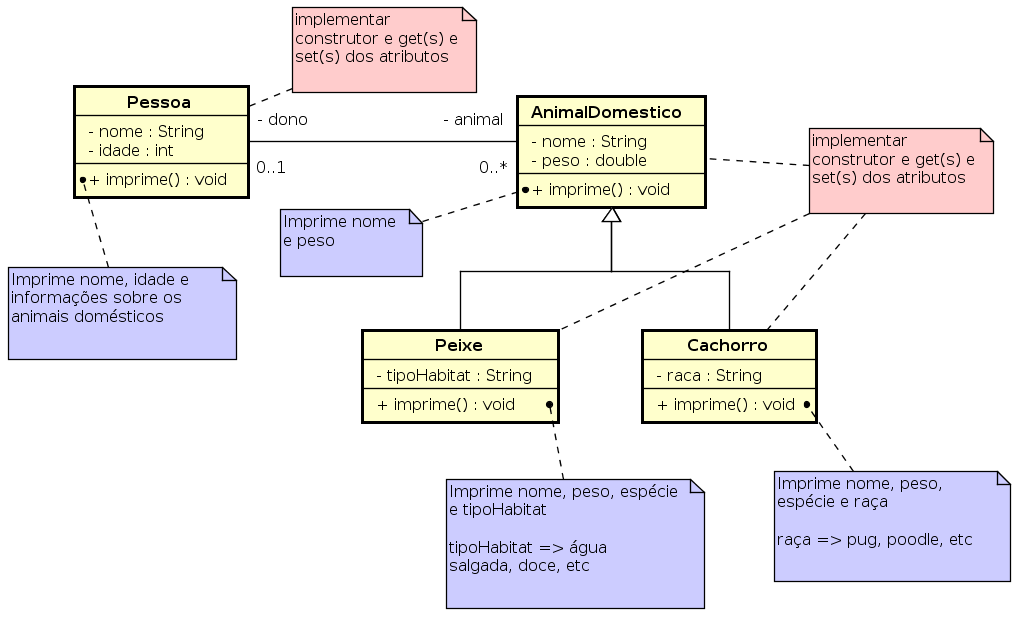
\includegraphics[width=15cm]{animal.png}
  \end{figure}
  
\section*{Classe {\sf Peixe} (subclasse de {\sf AnimalDomestico})}

\begin{itemize}

\item Atributos: tipoHabitat ({\sf string}) -- água doce, água salgada, etc

\item Construtor único que inicializa os atributos       

\item Métodos {\it getters/setters}

\item Método {\sf void imprime()} -- que imprime nome, peso, espécie e tipo de habitat

\end{itemize}

\section*{Classe {\sf Cachorro} (subclasse de {\sf AnimalDomestico})}

\begin{itemize}

\item Atributos: raça ({\sf string}) -- pug, poodle, etc

\item Construtor único que inicializa os atributos

\item Métodos {\it getters/setters}

\item Método {\sf void imprime()} -- que espécie, nome, peso, espécie e raça

\end{itemize}

\section*{Classe {\sf Pessoa}}

\begin{itemize}

\item Atributos: nome ({\sf string}), idade ({\sf int})
       
\item Métodos {\it getters/setters}

\item Método {\sf void imprime()} -- que imprime nome, idade e informações sobre os animais de estimação.

\item Métodos para adicionar e remover animais

\end{itemize}

\section*{Programa Principal}

Crie o arquivo {\sf main.cpp} com o seguinte conteúdo:

\par\noindent\rule{\textwidth}{0.4pt}

\begin{quote}
\begin{scriptsize}
\begin{verbatim}
#include "Peixe.h"
#include "Pessoa.h"
#include "Cachorro.h"
using namespace std;

int main(int argc, char** argv) {    
    Pessoa* pessoa = new Pessoa("Joao", 12);    
    Peixe* nemo = new Peixe("Nemo", 0.2, "Água salgada");
    Peixe* dory = new Peixe("Dory", 0.15, "Água doce");
    Cachorro* teo = new Cachorro("Teo", 6.2, "pug");
    
    pessoa->adiciona(nemo);    
    pessoa->adiciona(dory);        
    pessoa->adiciona(teo);
    
    pessoa->imprime();
    
    pessoa->remove("Dory");
    
    cout << endl;
    
    pessoa->imprime();

    // delete os objetos nemo, dory, teo e joao
    
    return 0;
}
\end{verbatim}
\end{scriptsize}
\end{quote}

\par\noindent\rule{\textwidth}{0.4pt}

\end{document}


